\chapter{Conclusion}
\label{chap:5}
Motivated by the examples of multi-agent systems in nature, we modelled a communication between two parent nodes and an agent node combining CTBN and POMDP frameworks. While the parent nodes emit messages containing information about their states, the agent observes a translation of these messages from which it needs to form its belief state and make decisions. The nodes evolve continuously in time as components of a CTBN, modelled as in \cref{sec:exp_ctbn_model}. Given that the messages of the parent nodes are unavailable to the agent, the interaction between the parent nodes and the agent node is modelled as POMDP, as described in \cref{sec:exp_pomdp_model}. We infer the observation model from simulated trajectories of nodes. \par
The belief state is updated utilising two methods. The first one is the exact update method, discussed in \cref{par:bs_exact}, and assumes that the transition intensities of the parents $ Q_1 $ and $ Q_2 $ are available for both the agent and the classifier. However, since this would not present a realistic system, particle filtering with marginalized CTBN is introduced as the state estimator. Given Gamma-priors of $ Q_1 $ and $ Q_2 $, the exact update method is well approximated by the marginal particle filter.\par
We consider this problem as a classification between observation models and analyze the performance of the classifier in terms of the metrics AUROC and AUPR. The results are given in \autoref{fig:AUROC_class0} and \autoref{fig:AUPR_class0}, respectively. Using the exact method to update the belief state, excellent performance is achieved for the classification task regarding AUROC metric. Since less information is available to the marginal particle filter, it yields a slightly lower performance, compared to the exact update method. Nevertheless, in both methods, as the number of samples increases, the metric approaches to 1, which is expected in the case of the unbiased classifier.\par
The results of the experiments with different levels of noise added to the observation model are given in \autoref{fig:AUROC_class0_error}. We assume that the noise level is available to the agent, and the likelihoods of noise-free observation models are considered for classification. Thus, the noisy model parameters are not estimated. The performance decreases as the noise introduced to the true observation model increases. These results confirm the expectations, as the noise leads to less reliable observations for the agent. On the other hand, with the increasing number of trajectories the metric converges to 1, showing robustness.\par
An important limitation to the inference task is the equivalence classes as introduced in \cref{sec:eq_classes}. The set of observation models can be divided into 10 equivalence classes such that the likelihoods of a sample trajectory $ S^{[0, T]} $ given any observation model within one class are equal. This situation limits the classifiers ability to determine the true model. Due to this limitation, the set of observation models is reduced to 10 observation models, each one representing an equivalence class. These observation models are given in \cref{eq:obs_set_exp}. Consequently, the result which states that the true observation model is $ \psi_i $ is equivalent to the one which states that the true observation model belongs to $ \text{i}^{\text{th}} $ equivalence class. As shown with examples in \cref{ap:eq_classes}, there are two reasons behind this equivalence. The first reason can be specified as the equivalent effect of observation models on the belief state, which is inherent to the observation model structure. The second reason is that the different belief states might lead to the same behaviour. This case can intuitively be explained by the fact that the agent may not need to use all the information it has for decision making. This information loss limits the ability to infer what the agent has observed from its actions.

\section{Outlook}
\label{chap:6}
A major step in the future is to eliminate the equivalence classes to be able to classify every observation model. This problem, to a certain extent, can be mitigated by joint inference of observation model and policy. The joint inference could be performed as a joint classification problem, where the combinations of discrete values of these parameters are treated as classes. This is only feasible by defining appropriate constraints on the policy such that, as for the case of observation models in this work, the policy space is countable. Another approach is to use function approximation to learn the observation model and the policy jointly.\par 
Another exciting direction is to employ our method in different environments to get insights into the interactions of agents and environments. 
Foerster \textit{et al.} \cite{Foerster2016} study a problem where the agents must learn to a communication protocol for information sharing to coordinate over a task. Our method can be utilised to infer and analyse the communication protocols that lead to the success or failure of the agents. For example, in the multi-step MNIST game, where the agents should agree on an encoding of digits, the encoding on which they have reached a consensus can be inferred. However, the problem needs simplifications to be feasible with our assumptions, i.e. only one acting agent. \par
%Another exciting direction is to solve the policy optimization problem, instead of assuming that the optimal policy is given. By doing so, it would be feasible to utilise the classification method for the observation model described in this work, in real-world data, providing insights into the interactions of agents and environments.\\
Moreover, it would be interesting to apply our model and solution approach to a more complex environment to evaluate the performance further. For example, one could experiment with non-binary messages, or more than two parent nodes.\par
%\begin{wrapfigure}{r}{6cm}
%	\begin{center}
%		\vspace{-13pt}
%		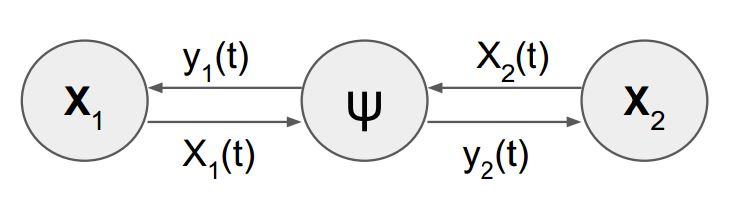
\includegraphics[width=5.5cm]{figures/multi-agent}
%		\caption[Multi-agent communication model]{Multi-agent communication model.}
%		\label{fig:multi_agent}
%	\end{center}
%\end{wrapfigure}

\begin{wrapfigure}{r}{6cm}
	\centering
	\vspace{20pt}
	\resizebox{.4\textwidth}{!}{
		\begin{tikzpicture}
		\tikzstyle{var} = [draw, circle, minimum size=1.2cm]
		\tikzstyle{line} = [draw, -latex]
		
		\node [var] (x1) {$X_1$};
		\node [var, right=1.5cm of x1] (psi) {$\psi$};
		\node [var, right=1.5cm of psi] (x2) {$X_2$};
		
		\path [line] ([yshift=3pt]x1.east) -- node[pos=0.5, above] {$ X_1(t) $} ([yshift=3pt]psi.west) ;
		\path [line] ([yshift=3pt]psi.east)  -- node[pos=0.5, above] {$ y_2(t) $} ([yshift=3pt]x2.west);
		\path [line] ([yshift=-3pt]x2.west) -- node[pos=0.5, below] {$ X_2(t) $} ([yshift=-3pt]psi.east) ;
		\path [line] ([yshift=-3pt]psi.west)  -- node[pos=0.5, below] {$ y_1(t) $} ([yshift=-3pt]x1.east);
		
		\end{tikzpicture}
	}
	\caption[Multi-agent communication model]{Multi-agent communication model.}
	\label{fig:multi_agent}
	%	\vspace{-8pt}
\end{wrapfigure}
In this thesis, we assume that the messages are relevant for a single node, and its actions affect merely its own dynamics. An extension to this model is to consider bidirectional communication between agents, as depicted in \autoref{fig:multi_agent}. In such communication, both nodes send messages, which are translated by the same observation model, and their behaviour depends on their observations and the belief states they keep. 

